\section{Data Quality Cuts and Signal Acceptance}
\label{secDataQualityCuts}

The peak processor in XERAWDP (see Section~\ref{secDAQ}) only provides peak candidates, and their selection is done in analysis. 
Parameters which are calculated based on the summed waveform (area [PE], height [mV], width [ADC bins], PMT coincidence level, delay time between S1 and S2, etc.) have been used to define cuts to ensure the data quality and to select only WIMP candidates. These cuts are grouped into the basic data quality cuts, consistency cuts, and the energy and single scatter section cuts. The acceptance of all cuts has been determined on the different data sets from the measurements, or on Monte Carlo simulations, and have been confirmed with the visual inspection of a large amount of events.



%{\bf Basic data quality cuts:}
\subsection{Basic Data Quality Cuts}
\label{secBasicCuts}
The waveforms which are not usable (due to muon interactions, micro-discharges, etc.) are rejected with the basic data quality cuts. \\
\\
{\bf `Signal-to-noise' cut (high energy event rejection):} \\
The area of the largest S1 and S2 peaks is compared to the area of the full waveform, in order to remove rare events due high energy (e.g. muon) interactions in the target volume, or micro-discharges on the cathode, which produce large amount of light, making it impossible to extract relevant information from the waveforms. The acceptance of the cut, determined on background data, is $>$96\% in the energy region of interest, and increases towards higher energies.
\\
\\
{\bf Hot spot cuts:}\\
During data acquisition, some PMTs occasionally show an unusual behavior: very large S2-like pulses only in one PMT, which are clearly uncorrelated to interactions in the target volume. The exact reason of these signals is not understood yet. However, they show very distinct features, which allows to cut such rare events. The acceptance has been computed on $^{241}$Am-Be calibration data as $>$99.6\%.



\subsection{Energy Cuts}
\label{secEnergyCuts}
These are are used to select events in the low energy region, where a WIMP signal is expected, and to ensure that they are not caused by PMT dark current are noise.
\\
\\
{\bf Software S2 threshold cut:}\\
The trigger efficiency starts to roll off for the summed S2 of both top and bottom PMT arrays below 300~PE (value before spatial corrections). In order to eliminate possible problems related to trigger efficiency, this cut requires the largest S2 peak in the trace to be above 300~PE. Due to charge losses caused by a finite electron lifetime, the acceptance of this cut is $Z$-dependent and increases with the increase of the electron lifetime. Charge losses are smaller closer to the liquid surface, thus the data from the top half of the target volume has been used to determine the acceptance of the cut, based on the measured S2 distribution for a given S1. During the data acquisition in the commissioning run in Fall 2009 (run07), the electron lifetime increased from 154~$\mu$s  to 192~$\mu$s, and from 230~$\mu$s to 380~$\mu$s during the 
first science run (run08). Taking into account these changes, the acceptance of the cut is 84\% at S1=4~PE, 95\% at S1=7~PE, and increases to 100\% at S1=14~PE. At energies higher than 13~PE the signal region is restricted to $-$3$\sigma$ quantile of the nuclear recoil band, and the corresponding acceptance loss is taken into account.
\\
\\
{\bf S1 coincidence level:}\\
For any valid S1 candidate, at least a 2-fold PMT coincidence in a 20~ns time window is required. This condition is necessary to avoid bias by electronic noise or PMT dark current. The acceptance of this cut, calculated with a Monte Carlo simulation, and is shown in Fig.~\ref{figCutCoincidence_1}. It is 97\% at S1 = 4~PE and increases to $>$99\% above S1 = 6~PE. 
This cut has been improved after unblinding the first science run data (see Section~\ref{secRun08}), which reduced the nuclear recoil acceptance by $<$0.4\%.

\begin{figure}[!h]
\centering
\subfigure[]{
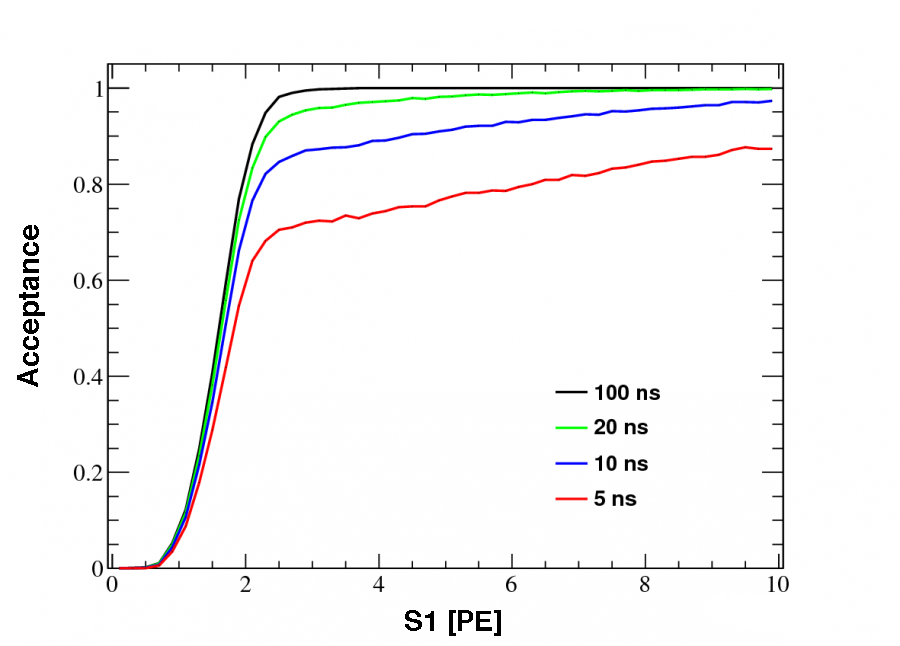
\includegraphics[height=0.33\linewidth]{plots/DataQualityCuts/S1coincidence_mod.png}
\label{figCutCoincidence_1}}
\subfigure[]{
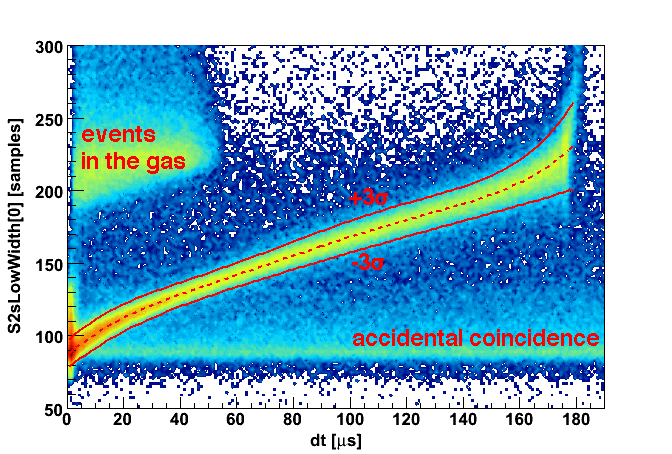
\includegraphics[height=0.33\linewidth]{plots/DataQualityCuts/S2width_Co60_mod.png}
\label{figCutCoincidence_2}}
\caption[Acceptance of S1 coincidence requirement, and the S2 signal width]{(a) - acceptance of S1 coincidence requirement, computed with a Monte Carlo simulation. A 2-fold coincidence in a 20~ns time window has been required in the run07 and run08 data analysis. Figure from Ref.~\cite{Guillaume}. (b) - width of the S2 signal as a function of the drift time. The `low width' parameter is measured at 10\% height of the S2 peak. Events in the gas phase with uncorrelated S1 and S2 are removed with a $\pm$3$\sigma$ cut.}
\label{figCutCoincidence}
\end{figure}


\subsection{Single Scatter Selection Cuts}
\label{secSingleScatterSelectionCuts}
Due to a very low WIMP-nucleon cross section, the dark matter particles are expected to interact with liquid xenon only once, whereas the $\gamma$-background often results in multiple vertices within the detector volume. Hence, several cuts are used to select single scatter interactions.
\\
\\
{\bf Single scatter events selection:}\\
Events with a single S2 are selected by a requirement of only one (largest) S2 peak. in order not not be biased by PMT after-pulses and single electron S2 signals, other S2 peak candidates are required to be smaller than a certain threshold ($\sim$100~PE), which depends on the size of the largest S2 peak. The acceptance of the cut of (95.1$\pm$2.9)\% has been determined on electronic recoil background data, which consists in the low energy region mostly of single scatter events.
\\
{\bf S1 noise cut:}\\
Due to the prompt nature of the scintillation signals, each particle interaction (both single and multiple scatters) will have only a single S1 peak in the trace. All other S1 candidates in a waveform are mostly from PMT dark current or mis-identified uncorrelated single electron S2 signals (see Fig.~\ref{figWaveform}). Pile-up is a very unlikely cause for such peaks, given the low event rate ($\sim$1~Hz) during acquisition of the dark matter data. Events with several S1 peaks are rejected when it cannot be clearly  decided, based on the drift time and a very conservative S2/S1 ratio, which S1 peak corresponds to the S2 signal. The acceptance of this cut has been determined on background data as (98.5$\pm$0.5)\%, and depends on the noise conditions during the measurement. Therefore, $\sim$20~days acquired in April 2010 had been rejected.
\\
\\
{\bf Veto coincidence cut:}\\
Events, in which a signal in the liquid xenon veto has been observed in coincidence with an S1 in the target volume, are rejected, as being due to $\gamma$-interactions. The energy threshold in the veto has been measured with a collimated $^{137}$Cs source (volume averaged value is 100~keV$_{\mathrm{ee}}$), as described in Section~\ref{secVetoEfficiencyMeasurement}. The acceptance of the veto coincidence cut, computed on a low energy background data, is $>$99.6\%.



\subsection {Consistency Cuts}
\label{secConsistencyCuts}
These cuts are targeted to remove events which pass the waveform analysis. They check if the topologies are consistent with the expectation for a single scatter interactions in the target volume, based on the width of the S2 signal, and based on S1 and S2 light patterns. \\
\\
{\bf S2 width cut:}\\
The width of S2 signal is energy dependent and increases with the depth of the interaction in the target volume, due to dispersion of the electron cloud during the drift towards the gas phase. A cut has been defined to check if the $Z$ coordinate inferred from the time delay between the S1 and S2 peaks is consistent with the width of the S2 peak. By definition, the acceptance of this cut, determined on $^{241}$Am-Be calibration data, is 90\%.
\\
\\
{\bf Position reconstruction quality cuts:}\\
Two cuts have been developed to ensure the quality of the position reconstruction and multiple scattering identifiation, where the individual interactions happen close in $Z$ and cannot be resolved by the peak finder. They are introduced and discussed in Section~\ref{secPosRecCuts}.
\\
\\
{\bf Anomalous event rejection:}

The S2 LCE is in general very good (see Section~\ref{secLCEs2}). However, in the region between the cathode and the bottom PMT window, which is 18~mm thick ($\sim$4~kg of liquid xenon), as well as between the PMTs of the bottom array, the electric field is reversed or absent. The ionization electrons from interactions in this region are drifted in the opposite direction and do not produce proportional scintillation signal (see Fig.~\ref{figGammaXtopology}). Therefore, this region is charge insensitive, and can be a source of so-called `gamma-X' events. Such events happen when a $\gamma$-ray has two or more interactions in the liquid xenon, at least one of which is in the region below the cathode. This results in a loss of some portion of the ionization signal, whereas scintillation produced in all interactions is detected, and leads to an abnormally low (non-Gaussian) value of the discrimination parameter log$_{10}$(S2/S1). Such events can mimic the nuclear recoil signal expected from a WIMP. 
%Multiple scattering events from electromagnetic background with one interaction in a charge insensitive volume (i.e. in the reverse field region below the cathode) have a signature of a single scattering event (one S1 and one S2 peak). However, part of the ionization signal is not detected, which leads to a lowered S2/S1 ratio, which can mimic a nuclear recoil and lead into potential leakage into the signal region.
The cut to reject such events is based on the likelihood ratio of the observed S1 hit pattern and the pattern expected from a calibration sample, for an interaction with the same coordinates. The acceptance of this cut, determined on $^{241}$Am-Be and $^{60}$Co calibration data, is (97.0$\pm$0.5)\%.

%\begin{floatingfigure}[r]{0.4\textwidth}
\begin{figure}[!h]
\centering
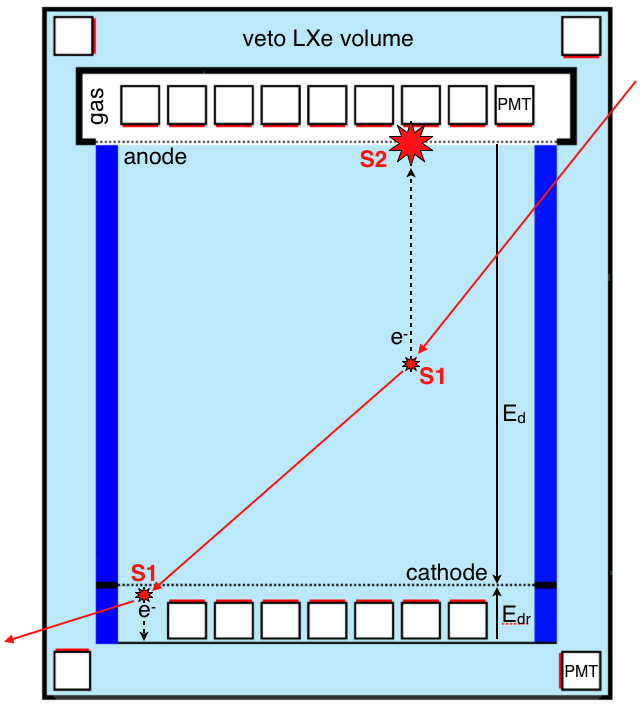
\includegraphics[width=0.4\linewidth]{plots/DataQualityCuts/GammaXtopology.png}
\caption[Topology of a `gamma-X' event]{Topology of a `gamma-X' event. If one or more interactions of a $\gamma$-ray are in the charge insensitive region below the cathode mesh, a portion of ionization signal is lost, which results in a lower S2/S1 ratio, which can mimic a nuclear recoil (WIMP) signature.}
\label{figGammaXtopology}
\end{figure}
%\end{floatingfigure}



\subsection{Signal Acceptance}
\label{secSignalAcceptance}

The cumulative acceptance of all data quality cuts is shown in Fig.~\ref{figCutsAcceptance}, together with the acceptance of the nuclear recoils due to the electronic recoil discrimination cut based on the S2/S1 ratio. The acceptance of the cuts used in the dark matter search analysis of the 11.17\% from the commissioning run in Fall 2009 (run07) from 60\% at 8.7~keV$_{\mathrm{nr}}$ to 85\% at 32.6~keV$_{\mathrm{nr}}$ (Fig.~\ref{figCutsAcceptance_2}), chosen as lower and upper bounds for the WIMP search energy range. The cumulative acceptance of the cuts used in the analysis of the first science run (run08) varies in the energy region 8.4$-$44.6~keV$_{\mathrm{nr}}$ from 61\% to 81\%. The upper energy bound has been extended in respect to the run07 analysis, in order to include most of the WIMP signal, as well for inelastic dark matter which is expected at higher energies~\cite{inelasticDM1, inelasticDM2}.

\begin{figure}[!h]
\centering
\subfigure[run07]{
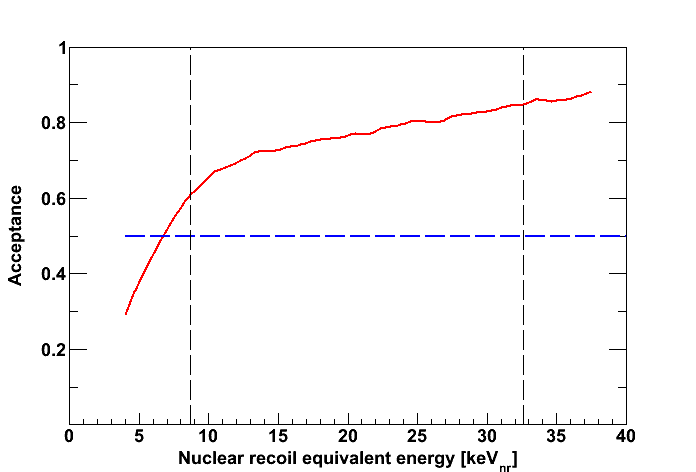
\includegraphics[width=0.475\linewidth]{plots/run07/run07_acceptance_modNoPE.png}
\label{figCutsAcceptance_1}}
\subfigure[run08]{
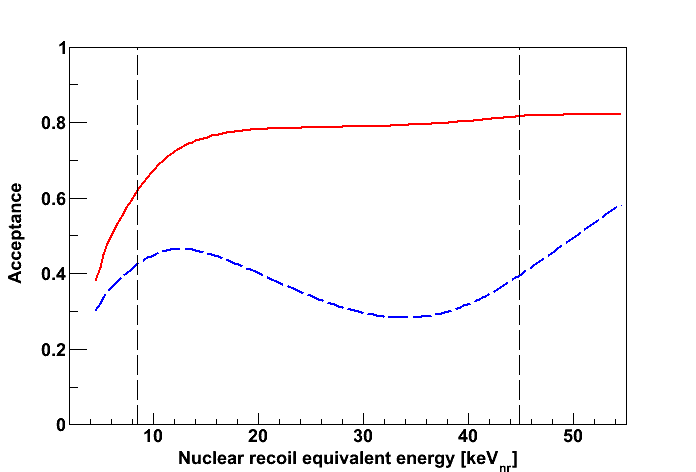
\includegraphics[width=0.475\linewidth]{plots/run08/run08_acceptance_modNoPE.png}
\label{figCutsAcceptance_2}}
\caption[Acceptance of all data quality cuts, excluding the S2/S1 discrimination, and nuclear recoil acceptance]{Acceptance of all data quality cuts (red) used for the analysis of the commissioning run (run07, (a)) and the first science run (run08, (b)) data, and nuclear recoil acceptance due to S2/S1 discrimination cut (blue). For the run07 analysis, a constant nuclear recoil acceptance of 50\% has been chosen. A constant 99.75\% electronic recoil rejection has been defined for the run08 analysis, which results in a slightly lower nuclear recoil acceptance. The vertical dashed lines indicate the WIMP-search energy regions in run07 and run08 analyses.}
\label{figCutsAcceptance}
\end{figure}

